\chapter{Testing}

\section{Overview}
At the start of the project, testing was to use two practices from Agile. These were Test Driven Development (TDD) and Continuous Integration (CI). Whilst these two practices both failed due to a mixture of reasons as described in the Iterations chapter, testing was still performed within each iteration. Rather than go over the tests made each week within the previous chapter, this section will summarise the testing. Overall there were 22 tests that tested the overall functionality of the system, see figure \ref{fig:test-output}. Unit tests were dropped for a number of reasons in favour of application tests.

Unit testing suits a situation where more of the base code is written by the developer, in this case the majority of the code is built on a pretested framework. Testing the final implementation would fit better than trying to test if a view is rendered by a controller correctly. Application tests can also be used to test the stories, meaning that they can give a much clearer indication of whether a story is complete and whether the end user will be happy. 

The time for extensive testing was also limited, meaning some tests had to be cut. The unit tests were the easiest to cut and seeing as the application tests tested the overall functionality of the system the lack of unit tests is not a terrible missing feature. 

\begin{figure}
	\caption{Output of the tests}
	\centerline{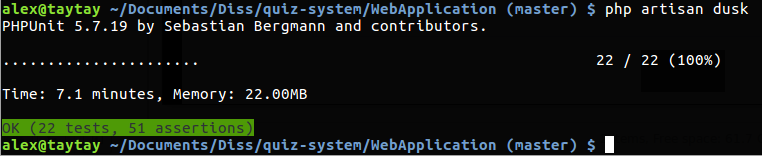
\includegraphics[scale=0.8]{Chapter4/test-output}}
	\label{fig:test-output}
\end{figure}

\section{Application testing}
To perform application tests, a testing framework called Laravel Dusk was used, which is the default testing framework provided with Laravel 5.4\cite{dusk}\cite{dusk-desc}. It runs the tests within a Chrome instance by running a standalone server which then calls the Chrome application installed on the machine that the tests are being run on. The advantages of running tests like this rather than say executing PHP on the server and reading a virtual DOM is that this allows JavaScript on the page to be evaluated and executed. JavaScript is vital to many of the components of the application so if it was not usable within tests, many parts of the system would have to be ignored within the tests.

These tests test the application as whole, rather than individual bits of code. This allows the tests to be written with the original requirements, the stories, in mind and so makes these tests a good way to evaluate the application at the end of its development. Tests were organised by story, as these provided an area of the application that needed to be checked, which makes them more human readable for any future development.

Tests use a test database rather than the production one to ensure the integrity of data on the production system. This test database is left intentionally empty, with each test performing a migration for the test. Within each test the database is populated with relevant data using a number of database factories. These factories allow the easy and quick creation of any data needed within the test, though using a normal Model to input data would also still work. At the end of each test, the database is rolled back for the next test to run, leaving an empty database for a new migration and data.

Database transactions could have been used instead, which use a pre migrated database and then any data input during each test is deleted at the end of the test. Whilst the test database could be migrated before any tests were run to allow the use of transactions, this would mean that any future changes to the migration files would mean that the developer would have to remember to re-migrate the test database as well. Doing a migration for every test might be somewhat resource intensive, but it allows the tests to be written and run completely standalone from each other with no need to tie into any earlier setup functions. 

\subsection{Limitations of dusk}
There were various problems encountered with Dusk throughout the project. These are likely due to the age of Dusk having only been released in January 2017. A major difficulty was that Dusk could not be run on Travis, the CI tool chosen for this project, which meant that CI had to be abandoned. The reasons for this are not understood, but it was better to run the tests manually than to spend a large amount of time trying to fix it, if at all possible.

As for the actual tests, there were a number of problems with the asserts and navigating pages that slowed how quickly tests could be written. The selectors in particular did not seem to all have the same functionality; some of them can take a HTML selector, similar to JQuery, where an HTML object could be selected by id or class. However, some could only be found by the name attribute and others by the content of the HTML tag and nothing else. The problems with lack of consistency was that a lot of assumptions were made about the way selectors worked, and the errors produced tended to simply say that the item being looked for was not found. This lead to a lot of frustration and confusion. 

Other problems with selectors included that they could not see inside iframes or canvas tags, a major part of showing results of quizzes. And if a selector did find a collection, it returned the first item on the page, and not a collection of items that can be iterated over. This problem in particular meant more work adding various unique ids or classes to items that were repeated on the page so that they could be selected without any issues.

There was additionally the issue that due to the amount of initial database seeding used within each test, the actual tests could get quite long in terms of line numbers. There was a lot of code repetition and this is something that could be improved upon in future by refactoring out some of the functionality into initialiser functions.

\section{Security testing}
\label{testing:security}
One story specifically concerns security: Users should not be able to submit their own answers by altering the HTML, as they did with Qwizdom. The tests for this however are not that easy to do within the confines of Dusk due to the nature of the framework. The framework is concerned with user facing application tests and has no ability to change the DOM of the page or send custom POST requests to the server. This means that this story is better tested in the user testing section.

Other aspects of security can be checked however, being a web application there are a number of well known attack types including SQL Injection, Cross-Site Scripting (XSS) and Cross-Site Request Forgery (CSRF) attacks. SQL injection attacks involves attackers trying to execute their own SQL code on the server, thereby giving them access to the system or to try and damage the system by say dropping some tables. XSS attacks are when attackers attempt to inject their own JavaScript into the system that may be run on another users page. Typically this would include injecting a script tag with malicious code into the database that would then be executed when written to the page by another user viewing a page. These tests are located in SecurityTest.php. There are five tests that test both SQL Injection and XSS attacks.  

For the SQL injection tests, a string that tries to insert a new database entry is used:
\begin{verbatim}
	"INSERT INTO `quizzes` 
		(`name`, `desc`, `user_id`, `created_at`, `updated_at`) 
		VALUES ('SQL Injection', 'this is an attack', '1', now(), now());"
\end{verbatim}
And for the XSS attacks it tries to add a script tag with an alert:
\begin{verbatim}
	<script>alert('hey xss');</script>
\end{verbatim} 

There are two main places that these attacks could be carried out. The first is on the front page, where the session search field could be used to insert malicious data. Though nothing is saved from this input, it does query the database, which means it could be subject to an SQL injection attack. If the search returned the original search query, then it could be used to embed some JavaScript, and if the search was then linkable (i.e. in the URL parameters), it could be sent on to other users. The other place that these two attacks could be carried out are on the admin backend, in the quiz and question creation pages where SQL or XSS code could be added to the body of the various quiz and question fields.

For SQL injection attacks, the easiest way to check that this data has not been added is to look for the record in the quizzes table. With the XSS attack, the page source can be searched for the script tag. Laravel copes with these attacks by default by escaping the inputs\cite{laravel-web-attacks}. With SQL, the entire string is quoted and not seen as an actual SQL command. With the XSS the HTML tags are escaped in a similar fashion, the \textless and \textgreater symbols are turned into \&lt; and \&gt; which are not rendered as HTML when written to the page\cite{laravel-web-attacks}.

The tests prove that the system works as intended and these two attack types are not possible. Cross site request forgery attacks are another form of attack but harder to test as they rely on the browsers weaknesses and come from another website. Dusk cannot simulate this sort of environment. However, for forms to be submitted within the system a CSRF token has to be submitted with the form. This token is compared to the user session to ensure they are the ones submitting this data, not a third party site. Laravel forces forms to contain this token, ensuring this attack cannot take place. 

\section{User testing}
At the end of development, the system was tested in a first year workshop, where they were asked to give feedback about the module. Feedback asked about their experience answering questions, viewing the graphs on the lecturers screen and the general user interface. The quiz was made by the lecturer beforehand rather than the developer, allowing some feedback from both a lecturer and the students. Feedback from students was split between those using mobile devices and desktops, with a larger number using desktops and two responses for mobile. The feedback from desktops was very positive, with all the responses rating four or five out of five regarding their experience. Although, there were comments that indicated a problem was lack of feedback when an answer was submitted, which would be an easy task for any further work.

As for mobile, the lack of responses make it difficult to tell what users thought. However the two responses received were split on their experiences. The first response indicated a somewhat positive experience, with a final rating of three out of five. The other response was much more negative, with a final rating of one. In the feedback about any bugs encountered it was stated that the quiz boxes were out of position and the wrong sizes. They also stated that they were using the default Samsung browser, which is not a browser that was tested on beforehand. Without knowing what the positive response was using, it is hard to tell if this is restricted to the Samsung browser. Mobile testing did use Chrome for Android which may be why this was missed as it appears like they behave differently.

Both mobile users also stated that the application did not update within a reasonable time, however this was not observed during development. This could be due to several reasons including bad Wifi signal in the lecture room or the devices themselves.

The lecturer for the session also gave some feedback based on their experience of using both the quiz creator and running the quiz in the workshop. The results indicated a generally positive experience, with all but one question receiving four or five out of ten. Just one question received a three out of five, which was how easy it was to run the quiz from the backend. There were also suggested additions and extensions. They stated their satisfaction by saying "Overall, very nice system that I think I could use."

For a more detailed breakdown of results, see appendix \ref{appendix:user-results}.

\section{Stress testing}
Though there are a number of tools out there to do exactly that, there was no time to set up and any official stress testing. However, the user tests within the lecture helped give an idea of the stress the system could take. It was able to support about twenty students connecting and answering questions without any issues. While the system is supposed to be up to 300, this is the best indicator at this point, and there were no problems.

\section{Automated testing}
Whilst CI was abandoned early on into the development of the application, the Dusk tests are easy to run and automatically execute within a browser if the appropriate browser drivers are available. This means that it should not be too hard to integrate these tests into a CI tool if required in any future development.